\documentclass[12pt]{article}

\usepackage{sbc-template}

\usepackage{graphicx,url}

\usepackage[brazil]{babel}   
%\usepackage[latin1]{inputenc}  
\usepackage[utf8]{inputenc}  
\usepackage{listings}
\usepackage{float}
% UTF-8 encoding is recommended by ShareLaTex

\usepackage{color}
\definecolor{javared}{rgb}{0.6,0,0} % for strings
\definecolor{javagreen}{rgb}{0.25,0.5,0.35} % comments
\definecolor{javapurple}{rgb}{0.5,0,0.35} % keywords
\definecolor{javadocblue}{rgb}{0.25,0.35,0.75} % javadoc

\lstset{language=Java,
	basicstyle=\ttfamily,
	keywordstyle=\color{javapurple}\bfseries,
	stringstyle=\color{javared},
	commentstyle=\color{javagreen},
	morecomment=[s][\color{javadocblue}]{/**}{*/},
	numbers=left,
	numberstyle=\tiny\color{black},
	stepnumber=1,
	numbersep=5pt,
	tabsize=2,
	showspaces=false,
	showstringspaces=false}
     
\sloppy

\title{Russia 2018 World Cup Route Using The Uniform Cost Method}

\author{Clovis Oliveira Mangueira\inst{1}, Fabrícia de Jesus Santos\inst{1}, \\ Paulo Victor dos Santos\inst{1}, 	Weslley Henrique Santos\inst{1}}


\address{Departamento de Sistemas de Informação \\Universidade Federal de Sergipe (UFS) -- Itabaiana, SE -- Brasil\\
  \email{\{clovis$\_$jack, paulo.victor$\_$18\}@hotmail.com}
  \email{fabriciacooper@gmail.com, weslley$\_$campos@outlook.com}
}

\begin{document} 

\maketitle

\section{Introdução}
No Brasil, o futebol é a paixão da nação e muitas vezes sendo considerado o esporte mais importante. Devido a essa paixão, a torcida brasileira é fiel ao seu time, desse modo, não seria diferente na copa do mundo. A copa do mundo está sendo realizada na Rússia, o qual é considerado o maior país de extensão territorial. 

O jogos são realizados em províncias (estados) diferentes com grande distância, o que consequentemente, leva muito tempo para viagem. Para facilitar o deslocamento e poder acompanhar melhor os jogos, o projeto tem como objetivo apresentar o melhor caminho para os amantes de futebol. Utilizando o método de custo uniforme, os critérios escolhidos para apresentar o melhor caminho, foram: distância, tempo e número de pedágio de um percusso.
\section{Busca de Custo Uniforme}
A estratégia de busca uniforme é uma pequena modificação da estratégia de busca em largura. Na busca em largura primeiro expande-se o nó raiz, depois todos os nós gerados por esse, e assim por diante até que se chegue ao estado meta. Ou seja, todos os nós que estão numa profundidade d da árvore serão expandidos e visitados antes que os nós que estão numa profundidade d+1.

A estratégia de busca uniforme é basicamente a mesma coisa. Mas ao invés de pegar o primeiro nó expandido que está na lista aguardando processamento, o nó que possui o menor custo (g(N)) será escolhido para ser expandido. Se certas condições sempre forem cumpridas, garante-se que a primeira solução encontrada será a mais barata. Uma condição é a seguinte: o custo do caminho nunca deve ir diminuindo conforme avançamos por ele, em outras palavras, é importante que:
\begin{lstlisting}[caption = Pseudo-código para calcular a função g(n)]
g(Sucessor)>=g(N)	
em todos os nos N, 
g(N) e o custo conhecido de ir-se da raiz ate o nodulo N.
\end{lstlisting}

\section{Aplicação}
A aplicação se baseou com dados fornecido por uma empresa russa Astra Log. A mesma é uma empresa que oferece serviços de transporte de mercadoria para vários países, principalmente a Rússia. Logo, foi possível gerar o grafo para ajudar no desenvolvimento do projeto. Pode-se acompanhar o grafo na \ref{fig:fig1}, onde cada ponto representa as cidades que acontecerão os jogos para a copa do mundo. Dentro dos dados fornecidos pela empresa Astra Log, estava a distancia de uma cidade para outra. Porém, para obter o tempo e o número de pedágio, realizou-se uma busca no Google Maps. 
\begin{figure}[h]
	\centering
	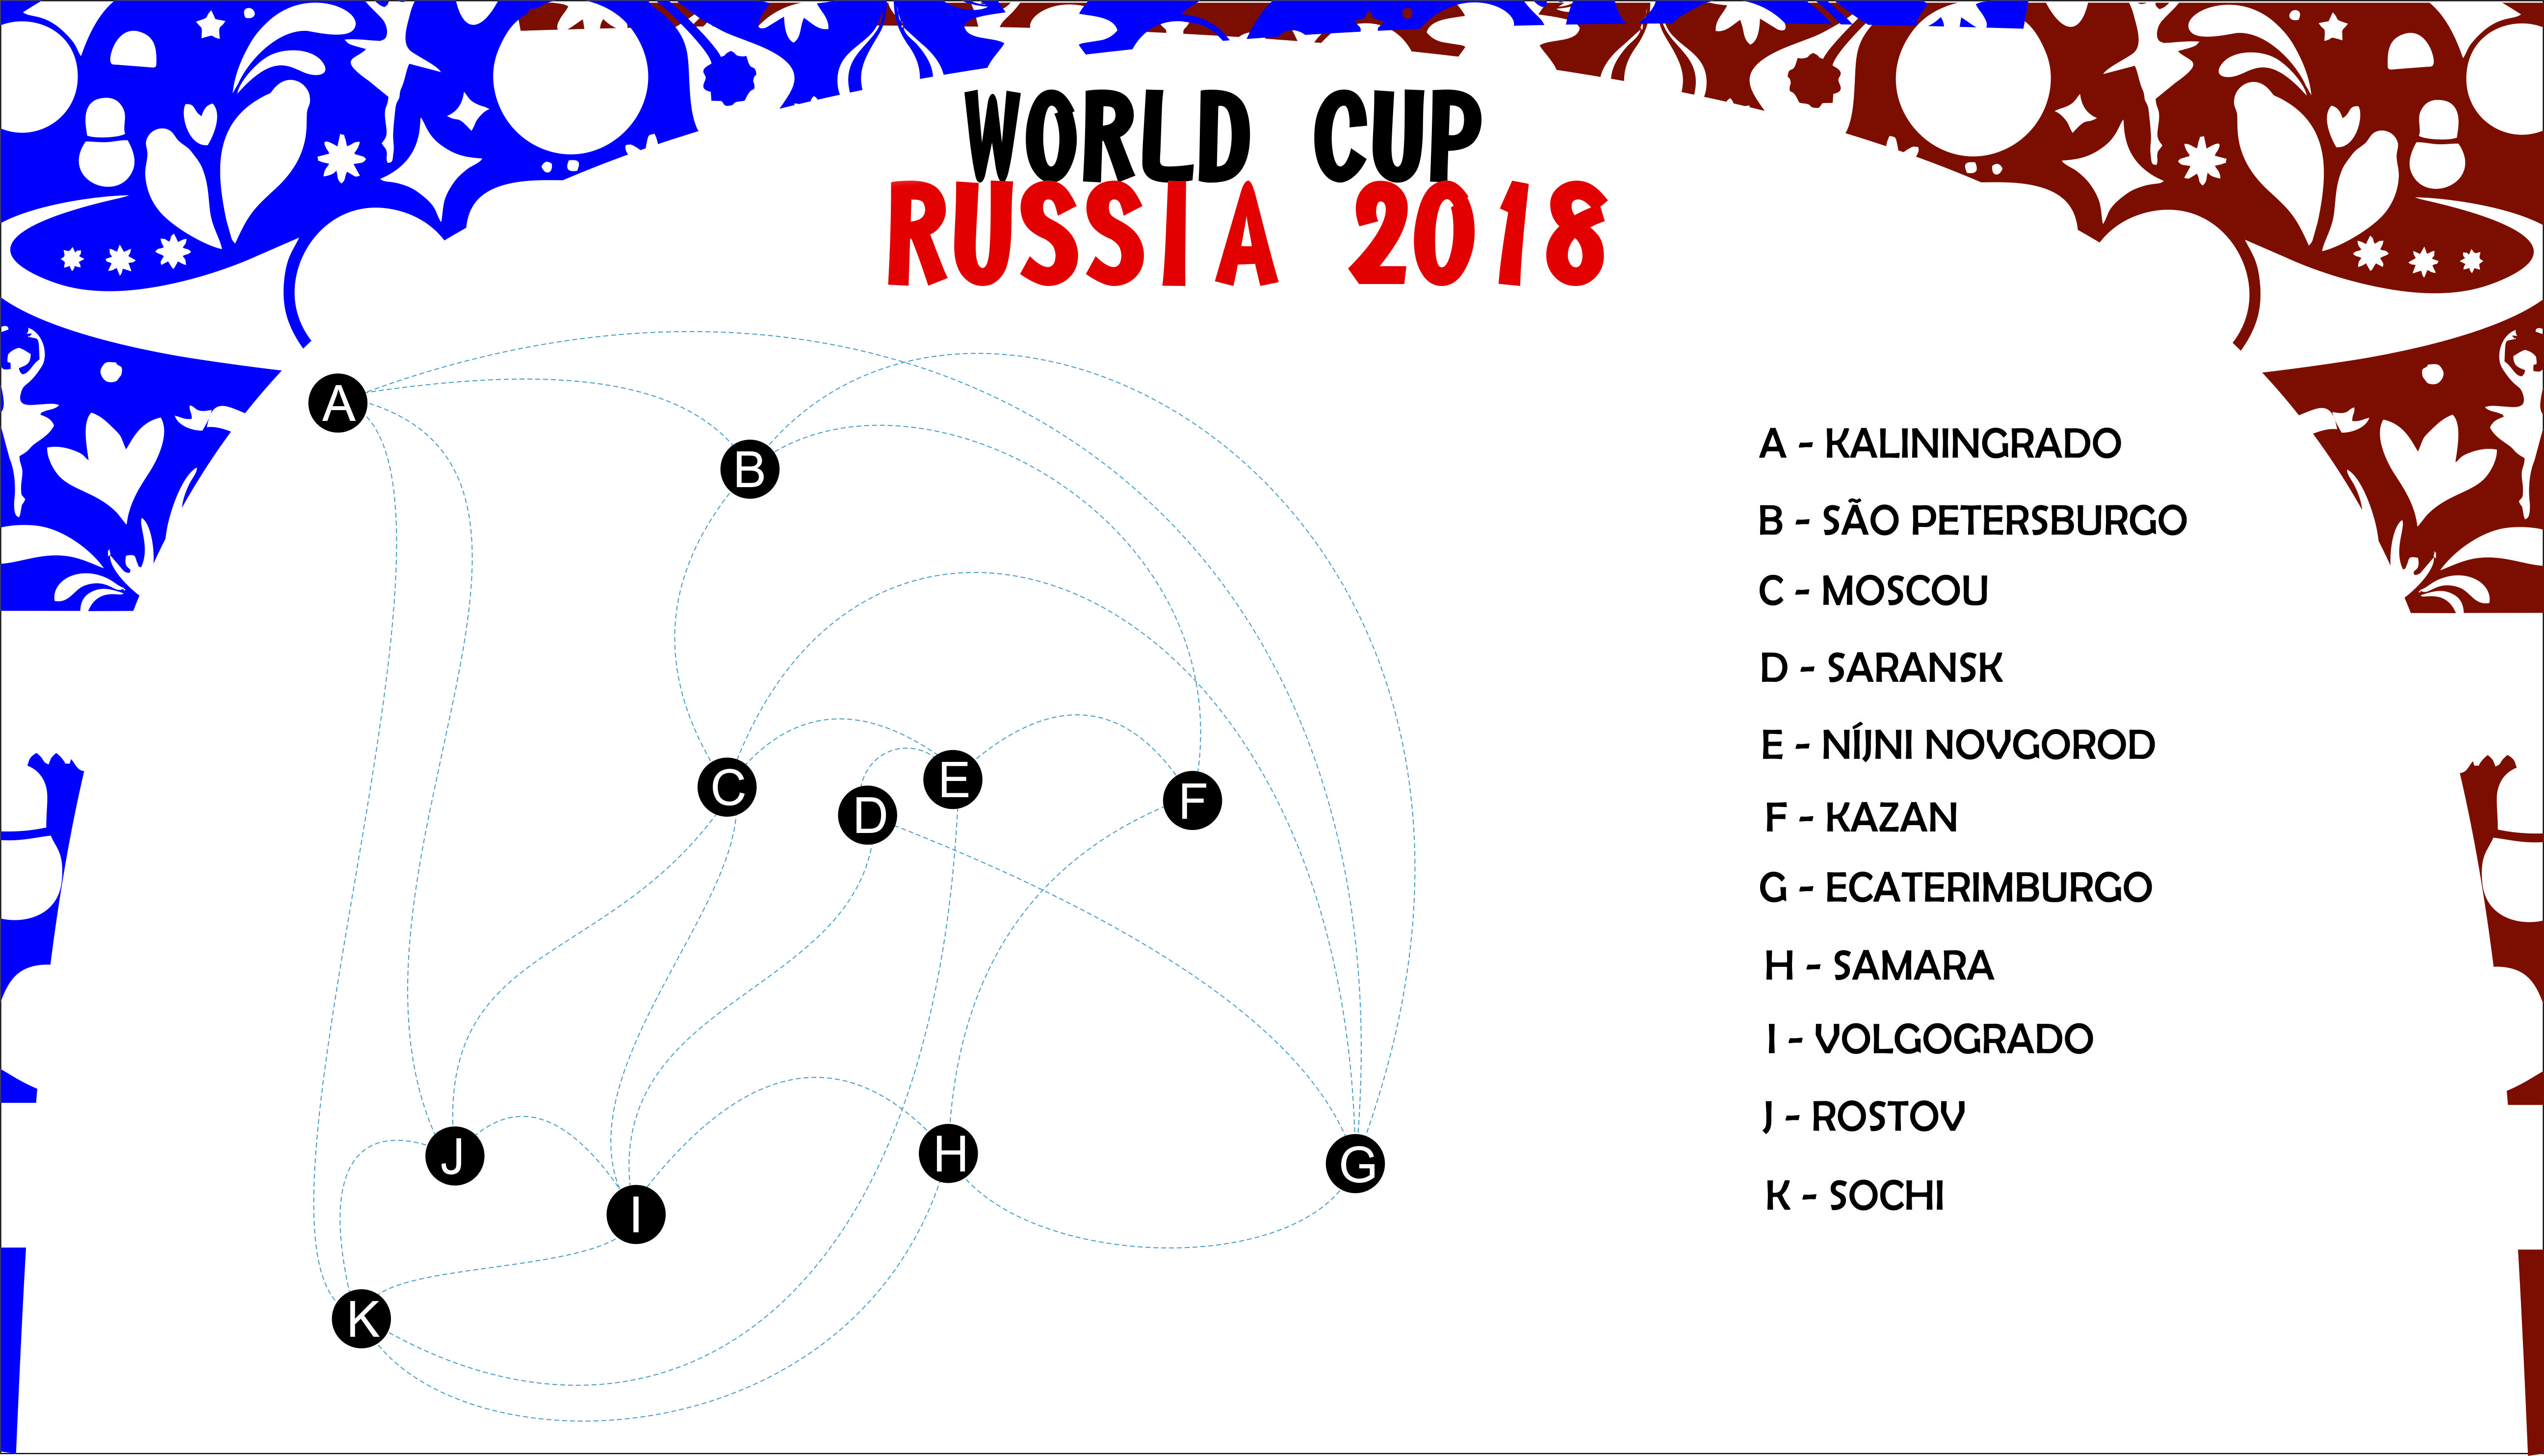
\includegraphics[width=0.9\columnwidth]{imagem/GRAFO}
	\caption{Grafo}
	\label{fig:fig1}
\end{figure}
Contudo, a aplicação tem por objetivo mostrar para ao usuário o melhor caminho entre as cidades que irão acontecer os jogos, onde dado um estado de partida e um de destino, o programa irá traçar um caminho com base nas informações definidas, que compõe a função G, sendo elas distância, tempo e a número de pedágios dentro da rota.
\subsection{Implementação}
Com os dados definidos, inicialmente, efetuou uma normalização dos dados para equilibrar os seus valores. Essa normalização se dá pela fórmula: \[ g(X) = \frac{x - min}{max - min} \]. Onde:
\begin{enumerate}
	\item x é o valor que deseja normalizar;
	\item $min$ representa o valor mínimo dentre os vértices;
	\item $max$ representa o valor máximo dentre os vértices;
	\item g(X) equivale ao valor normalizado. 
\end{enumerate}

Em seguida, temos o método principal do projeto. Basicamente, dada uma origem e destino, o primeiro elemento será adicionado na fila. Nesse caso o primeiro elemento será o ponto de origem. Se a fila não estiver vazia, a variável ``cidadePai''do tipo ``Cidade'' guarda o primeiro elemento da fila. Como forma de controle, uma condição foi criada para saber se a cidade de origem e destino fossem iguais, caso fosse o método retornaria a cidade atual. Senão, um laço de repetição foi criado para varrer a matriz criada e buscar quais nós não eram visitados e que a matriz não retornasse um valor 0 --- se retornar valor 0 era porque não tinha encontrado nenhuma adjacência. Logo se a condição fosse verdadeira, os custos seriam somados ao longo do laço e cada cidade seria adicionada na fila para comparações futuras, até que a condição fosse falsa. 
\begin{lstlisting} [caption= Método Principal do Projeto]
public Cidade uniformCustSearch(int origem, int destino) {

	PriorityQueue<Cidade> fila = new PriorityQueue<Cidade>();
	cidades[destino].setIsFinal(true);
	cidades[origem] .setWasVisited(true);
	fila.add(cidades[origem]);
	
	while (!fila.isEmpty()) {
	
		Cidade cidadePai = fila.remove();
		
		if (cidadePai.isFinal() == cidades[destino].isFinal())
		return cidadePai;
		
		for (int cidadeAtual = 0; 
		cidadeAtual < matriz_adjacente.length; 
		cidadeAtual++) {
			if ((matriz_adjacente[cidadePai.getPosition()][cidadeAtual] != 0)
			 && (cidades[cidadeAtual].wasVisited() == false)) {
				cidades[cidadeAtual].setCustNode(cidadePai.getCustNode() 
				+ matriz_adjacente[cidadePai.getPosition()][cidadeAtual]);
				cidades[cidadeAtual].setPai(cidades[cidadePai.getPosition()]);
				cidades[cidadeAtual].setWasVisited(true);
				fila.add(cidades[cidadeAtual]);
			}
		}
	}
	return null;
}
\end{lstlisting}
\subsection{Interface}
Para saber qual melhor caminho, o usuário deve selecionar sua origem e seu destino comboBox, localizado no canto direito da tela. A partir desse momento, ao clicar no botão iniciar, a aplicação irá apresentar o melhor caminho, mostrando os pontos das cidades a serem passadas. Logo a baixo segue a imagem \ref{fig:fig2}.
\begin{figure}[H]
	\centering
	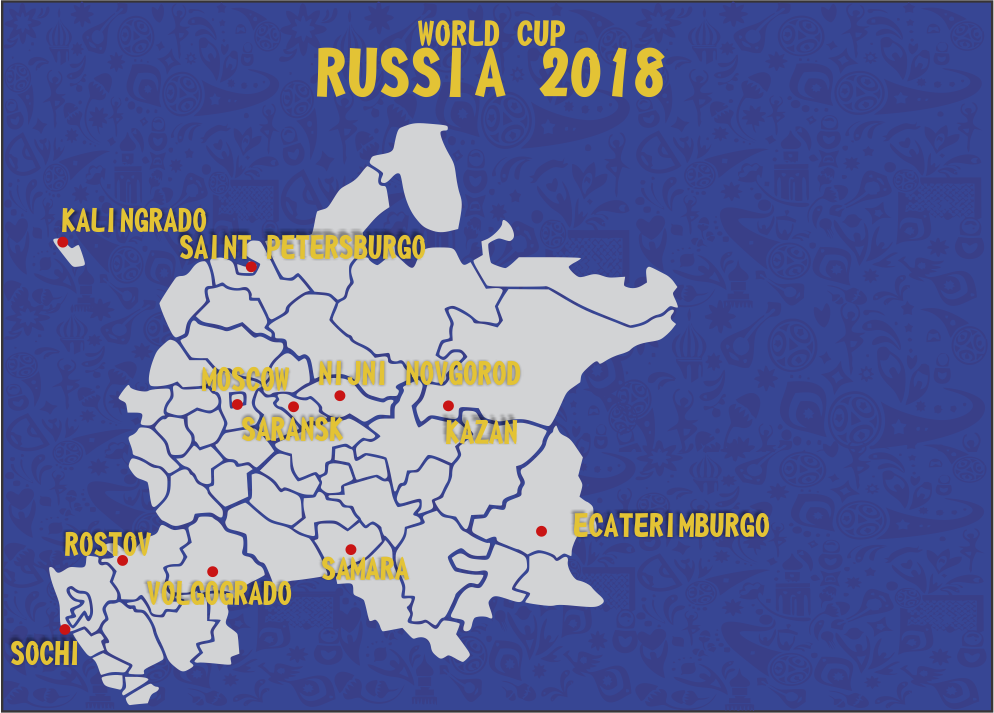
\includegraphics[width=0.9\columnwidth]{imagem/TELAESBOCO}
	\caption{Tela Inicial}
	\label{fig:fig2}
\end{figure}

%colocar imagem da interface
\section{Conclusão}
O presente projeto teve por objetivo aplicar o algoritmo de busca de custo uniforme sobre o problema citado anteriormente. O maior propósito é ganhar conhecimento sobre a área de Inteligência Artificial e ter suporte para aplicar os seus conceitos. Contudo, o método de busca do custo uniforme, não realiza a busca de uma forma ótima, já que ele tem um grande custo computacional, pois é necessário percorrer todos os nós da árvore, uma vez que o menor caminho mostrado por ele, não será de fato o menor.
\end{document}
